36. $\cfrac{(x+1)\sqrt{-x^2-10x+11}}{x^2+x-12}\geqslant0\Leftrightarrow \cfrac{(x+1)\sqrt{-(x+11)(x-1)}}{(x+4)(x-3)}\geqslant0.$ Применив метод интервалов, найдём ответ: $x\in\{-11;1\}\cup(-4;-1].$
\begin{figure}[ht!]
\center{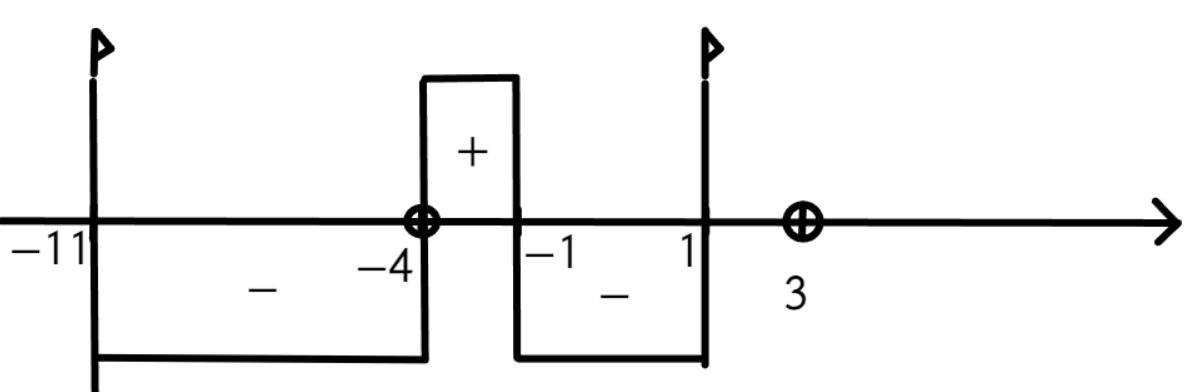
\includegraphics[scale=0.35]{ner9-36.png}}
\end{figure}\\
